\chapter{Machine Learning: Introduction}

\begin{customArrayStretch}{1.5}
\begin{longtable}{l p{7cm}}

\hline\endfirsthead
\hline\endhead
\hline\endfoot
\hline
\caption*{Notations} \\
\endlastfoot

$N$ & number of training records\\ \hline

$\dCurlyBrac{\bm{x}_1, \cdots , \bm{x}_N }$ & input records \\ \hline

$\dCurlyBrac{\bm{y}_1, \cdots , \bm{y}_N }$ & (ground truth/ reference) outputs \\ \hline

$\bm{y}(\cdot)$ & model/ function \\ \hline

$\hat{\bm{y}}_i = \bm{y}(\bm{x_i})$ & (hypothesis) output of $i$-th input \\



\end{longtable}
\end{customArrayStretch}


\section{Intro}

\begin{enumerate}
    \item In practical applications, the variability of the input vectors will be such that the training data can comprise only a tiny fraction of all possible input vectors, and so generalization is a central goal in pattern recognition.
    \hfill \cite{ml/book/Pattern-Recognition-And-Machine-Learning/Christopher-M-Bishop}
\end{enumerate}





\section{Pre-processing: Feature Extraction}

\begin{enumerate}
    \item For most practical applications, the original input variables are typically preprocessed to transform them into some new space of variables where, it is hoped, the pattern recognition problem will be easier to solve.
    \hfill \cite{ml/book/Pattern-Recognition-And-Machine-Learning/Christopher-M-Bishop}

    \item Pre-processing might also be performed in order to speed up computation.
    \hfill \cite{ml/book/Pattern-Recognition-And-Machine-Learning/Christopher-M-Bishop}

    \item Care must be taken during pre-processing because often information is discarded, and if this information is important to the solution of the problem then the overall accuracy of the system can suffer.
    \hfill \cite{ml/book/Pattern-Recognition-And-Machine-Learning/Christopher-M-Bishop}
\end{enumerate}




\section{Training/ Learning Phase}

\begin{enumerate}
    \item \textbf{Training set}: large set of $N$ records $\dCurlyBrac{\bm{x}_1, \cdots , \bm{x}_N }$ that can be used to tune the parameters of an adaptive model.
    \hfill \cite{ml/book/Pattern-Recognition-And-Machine-Learning/Christopher-M-Bishop}

    \item The result of running the machine learning algorithm can be expressed as a function $\bm{y}(\bm{x}_i)$ which takes a new input record $\bm{x}$ as input and that generates an output vector $\bm{y}_i$, encoded in the same way as the target vectors.
    The precise form of the function $\bm{y}(\cdot)$ is determined during the training phase, also known as the learning phase, on the basis of the \textbf{training data}.
    \hfill \cite{ml/book/Pattern-Recognition-And-Machine-Learning/Christopher-M-Bishop}
\end{enumerate}



\section{Testing/ Evaluation Phase}

\begin{enumerate}
    \item Once the model is trained it can then determine the identity of new digit images, which are said to comprise a \textbf{test set}.
    \hfill \cite{ml/book/Pattern-Recognition-And-Machine-Learning/Christopher-M-Bishop}

    \item The ability to categorize correctly new examples that differ from those used for training is known as \textbf{generalization}.
    \hfill \cite{ml/book/Pattern-Recognition-And-Machine-Learning/Christopher-M-Bishop}
\end{enumerate}





\section{Supervised learning}

\begin{enumerate}
    \item Applications in which the training data comprises examples of the input vectors along with their corresponding target vectors are known as \textbf{supervised learning} problems.
    \hfill \cite{ml/book/Pattern-Recognition-And-Machine-Learning/Christopher-M-Bishop}
\end{enumerate}



\subsection{Regression}

\begin{enumerate}
    \item Cases in which the desired output consists of one or more continuous variables, then the task is called \textbf{regression}.
    \hfill \cite{ml/book/Pattern-Recognition-And-Machine-Learning/Christopher-M-Bishop}
\end{enumerate}


\subsection{Classification}

\begin{enumerate}
    \item Cases in which the aim is to assign each input vector to one of a finite number of discrete categories, are called \textbf{classification} problems.
    \hfill \cite{ml/book/Pattern-Recognition-And-Machine-Learning/Christopher-M-Bishop}
\end{enumerate}





\section{Unsupervised learning}

\begin{enumerate}
    \item the training data consists of a set of input vectors $\bm{x}$ without any corresponding target values
    \hfill \cite{ml/book/Pattern-Recognition-And-Machine-Learning/Christopher-M-Bishop}
\end{enumerate}

\subsection{Clustering}

\begin{enumerate}
    \item Cases to discover groups of similar examples within the data
    \hfill \cite{ml/book/Pattern-Recognition-And-Machine-Learning/Christopher-M-Bishop}
\end{enumerate}


\subsection{Density Estimation}

\begin{enumerate}
    \item Cases to determine the distribution of data within the input space
    \hfill \cite{ml/book/Pattern-Recognition-And-Machine-Learning/Christopher-M-Bishop}
\end{enumerate}


\subsection{Visualization}

\begin{enumerate}
    \item Cases to project the data from a high-dimensional space down to two or three dimensions
    \hfill \cite{ml/book/Pattern-Recognition-And-Machine-Learning/Christopher-M-Bishop}
\end{enumerate}


\section{Reinforcement Learning}

\begin{enumerate}
    \item It is concerned with the problem of finding suitable actions to take in a given situation in order to maximize a reward.
    \hfill \cite{ml/book/Pattern-Recognition-And-Machine-Learning/Christopher-M-Bishop}

    \item Here the learning algorithm is not given examples of optimal outputs, in contrast to supervised learning, but must instead discover them by a process of trial and error.
    \hfill \cite{ml/book/Pattern-Recognition-And-Machine-Learning/Christopher-M-Bishop}

    \item Typically there is a sequence of states and actions in which the learning algorithm is interacting with its environment.
    \hfill \cite{ml/book/Pattern-Recognition-And-Machine-Learning/Christopher-M-Bishop}

    \item In many cases, the current action not only affects the immediate reward but also has an impact on the reward at all subsequent time steps.
    \hfill \cite{ml/book/Pattern-Recognition-And-Machine-Learning/Christopher-M-Bishop}

    \item \textbf{Credit assignment problem}:
    \hfill \cite{ml/book/Pattern-Recognition-And-Machine-Learning/Christopher-M-Bishop}
    \begin{enumerate}
        \item A major challenge is that a case can involve dozens of moves, and yet it is only at the end of the case that the reward, in the form of victory, is achieved.
        \hfill \cite{ml/book/Pattern-Recognition-And-Machine-Learning/Christopher-M-Bishop}

        \item The reward must then be attributed appropriately to all of the moves that led to it, even though some moves will have been good ones and others less so.
        \hfill \cite{ml/book/Pattern-Recognition-And-Machine-Learning/Christopher-M-Bishop}
    \end{enumerate}

    \item A general feature of reinforcement learning is the trade-off between \\
    \textbf{exploration}, in which the system tries out new kinds of actions to see how effective they are, and \\
    \textbf{exploitation}, in which the system makes use of actions that are known to yield a high reward.
    \hfill \cite{ml/book/Pattern-Recognition-And-Machine-Learning/Christopher-M-Bishop}

    \item Too strong a focus on either exploration or exploitation will yield poor results.
    \hfill \cite{ml/book/Pattern-Recognition-And-Machine-Learning/Christopher-M-Bishop}
\end{enumerate}









\section{Model Comparison OR Model Selection}

\begin{enumerate}
    \item A bad model can cause \textit{overfitting} or \textit{underfitting} and sometimes even lead to increased computational costs.
    \hfill \cite{geeksforgeeks/machine-learning/model-selection-for-machine-learning}

    \item Different models have different ways of processing data and choosing the right one ensures that the system works efficiently.
    \hfill \cite{geeksforgeeks/machine-learning/model-selection-for-machine-learning}
    \begin{enumerate}
        \item A simple model cannot capture details and has poor accuracy, while a model too complex might overfit that is doing very well on training data but fails on new data.
        \hfill \cite{geeksforgeeks/machine-learning/model-selection-for-machine-learning}

        \item The goal is to find a model that learns patterns effectively without being too simple or too complex.
        \hfill \cite{geeksforgeeks/machine-learning/model-selection-for-machine-learning}
    \end{enumerate}

    \item Proper model selection involves experimenting with different models and comparing their performance using evaluation metrics such as accuracy, precision, recall or mean squared error.
    These metrics help in determining which model is best suited for a given task.
    \hfill \cite{geeksforgeeks/machine-learning/model-selection-for-machine-learning}

    \item Apart from performance metrics, other factors such as training time, dataset size and available computing power also play a crucial role in choosing the right model.
    \hfill \cite{geeksforgeeks/machine-learning/model-selection-for-machine-learning}

    \item Selecting an appropriate model not only improves prediction accuracy but also enhances efficiency, making the system faster and more reliable.
    \hfill \cite{geeksforgeeks/machine-learning/model-selection-for-machine-learning}
\end{enumerate}




\subsection{Grid Search}

\begin{enumerate}
    \item One of the simplest and most commonly used model selection techniques
    \hfill \cite{geeksforgeeks/machine-learning/model-selection-for-machine-learning}

    \item In this approach, systematically different combinations of hyper-parameters are tried and that gives the best performance chosen.
    \hfill \cite{geeksforgeeks/machine-learning/model-selection-for-machine-learning}

    \item It can be effective, but the main drawback will be computationally intensive, especially for complex models and many parameters.
    \hfill \cite{geeksforgeeks/machine-learning/model-selection-for-machine-learning}
\end{enumerate}



\subsection{Random Search}

\begin{enumerate}
    \item Similar to grid search, random search doesn't check all possible combinations. Instead, it randomly chooses a subset of the hyperparameter combinations.
    \hfill \cite{geeksforgeeks/machine-learning/model-selection-for-machine-learning}

    \item The random search method often runs much faster than the grid search method and yet achieves equally good results.
    \hfill \cite{geeksforgeeks/machine-learning/model-selection-for-machine-learning}
\end{enumerate}



\subsection{Bayesian Optimization}

\begin{enumerate}
    \item Bayesian optimization is a smarter approach to model selection.
    \hfill \cite{geeksforgeeks/machine-learning/model-selection-for-machine-learning}

    \item Instead of just randomly searching for the best hyper-parameters, it uses probability models to predict which parameters are likely to perform best and focuses on evaluating those.
    \hfill \cite{geeksforgeeks/machine-learning/model-selection-for-machine-learning}

    \item This method is efficient and often finds better results than grid or random search.
    \hfill \cite{geeksforgeeks/machine-learning/model-selection-for-machine-learning}
\end{enumerate}



\subsection{Cross-Validation Based Selection}

\begin{enumerate}
    \item This method involves using cross-validation to evaluate multiple models and selecting the one with the best average performance.
    \hfill \cite{geeksforgeeks/machine-learning/model-selection-for-machine-learning}

    \item Instead of relying on a single train-test split, cross-validation divides the dataset into multiple parts and trains the model on different subsets.
    This helps to ensure that the model’s performance is not just due to a specific split of data.
    \hfill \cite{geeksforgeeks/machine-learning/model-selection-for-machine-learning}

    \item By averaging the results from different splits, we get how well the model will perform on new, unseen data.
    \hfill \cite{geeksforgeeks/machine-learning/model-selection-for-machine-learning}

    \item This approach reduces the risk of overfitting and helps in selecting a good model.
    \hfill \cite{geeksforgeeks/machine-learning/model-selection-for-machine-learning}
\end{enumerate}




\subsubsection{Holdout Validation}

\begin{enumerate}
    \item In Holdout Validation we perform training on the 50\% of the given dataset and rest 50\% is used for the testing purpose.
    \hfill \cite{geeksforgeeks/machine-learning/cross-validation-machine-learning}

    \item It's a simple and quick way to evaluate a model.
    \hfill \cite{geeksforgeeks/machine-learning/cross-validation-machine-learning}

    \item The major drawback of this method is that we perform training on the 50\% of the dataset, it may possible that the remaining 50\% of the data contains some important information which we are leaving while training our model that can lead to higher bias.
    \hfill \cite{geeksforgeeks/machine-learning/cross-validation-machine-learning}
\end{enumerate}



\subsubsection{LOOCV (Leave One Out Cross Validation)}

\begin{enumerate}
    \item In this method we perform training on the whole dataset but leaves only one data-point of the available dataset and then iterates for each data-point.
    \hfill \cite{geeksforgeeks/machine-learning/cross-validation-machine-learning}

    \item In LOOCV the model is trained on $n-1$ samples and tested on the one omitted sample repeating this process for each data point in the dataset.
    \hfill \cite{geeksforgeeks/machine-learning/cross-validation-machine-learning}

    \item An advantage of using this method is that we make use of all data points and hence it is low bias.
    \hfill \cite{geeksforgeeks/machine-learning/cross-validation-machine-learning}

    \item The major drawback of this method is that it leads to higher variation in the testing model as we are testing against one data point. If the data point is an outlier it can lead to higher variation.
    \hfill \cite{geeksforgeeks/machine-learning/cross-validation-machine-learning}

    \item Another drawback is it takes a lot of execution time as it iterates over the number of data points we have.
    \hfill \cite{geeksforgeeks/machine-learning/cross-validation-machine-learning}
\end{enumerate}





\subsubsection{Stratified Cross-Validation}

\begin{enumerate}
    \item It is a technique used in machine learning to ensure that each fold of the cross-validation process maintains the same class distribution as the entire dataset. 
    \hfill \cite{geeksforgeeks/machine-learning/cross-validation-machine-learning}
    
    \item This is particularly important when dealing with \textbf{imbalanced datasets} where certain classes may be under represented. 
    \hfill \cite{geeksforgeeks/machine-learning/cross-validation-machine-learning}
    
    \item In this method:
    \begin{enumerate}
        \item The dataset is divided into k folds while maintaining the proportion of classes in each fold.
        \hfill \cite{geeksforgeeks/machine-learning/cross-validation-machine-learning}
        
        \item During each iteration, one-fold is used for testing and the remaining folds are used for training.
        \hfill \cite{geeksforgeeks/machine-learning/cross-validation-machine-learning}
        
        \item The process is repeated k times with each fold serving as the test set exactly once.
        \hfill \cite{geeksforgeeks/machine-learning/cross-validation-machine-learning}
    \end{enumerate}

    \item Stratified Cross-Validation is essential when dealing with classification problems where maintaining the balance of class distribution is crucial for the model to generalize well to unseen data.
    \hfill \cite{geeksforgeeks/machine-learning/cross-validation-machine-learning}
\end{enumerate}


\subsubsection{K-Fold Cross Validation }

\begin{figure}[H]
    \centering
    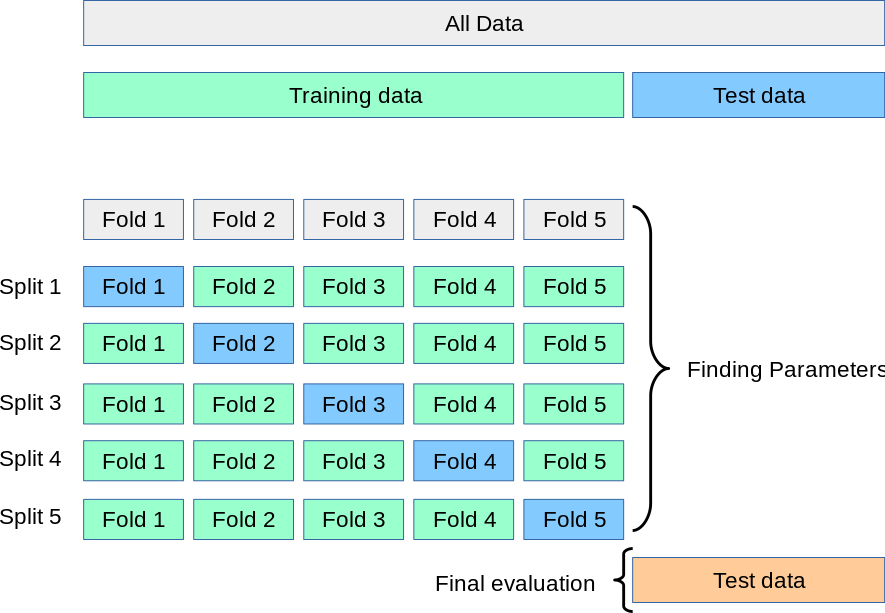
\includegraphics[
        width=\linewidth,
        height=5cm,
        keepaspectratio,
    ]{images/machine-learning/k-fold-cross-val.png}
\end{figure}

\begin{enumerate}
    \item In K-Fold Cross Validation we split the dataset into $k$ number of subsets known as folds then we perform training on the all the subsets but leave one ($k-1$) subset for the evaluation of the trained model. 
    \hfill \cite{geeksforgeeks/machine-learning/cross-validation-machine-learning}
    
    \item In this method, we iterate $k$ times with a different subset reserved for testing purpose each time.
    \hfill \cite{geeksforgeeks/machine-learning/cross-validation-machine-learning}
\end{enumerate}

















\section{Bias-Variance Trade Off}

\begin{figure}[H]
    \centering
    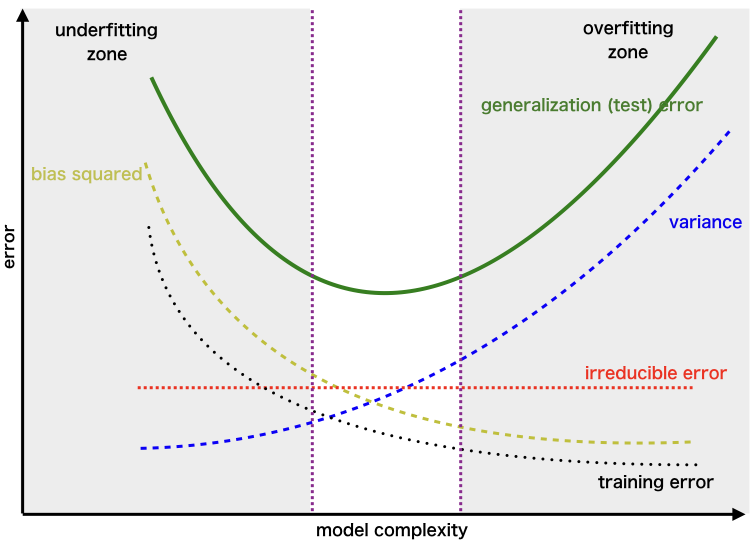
\includegraphics[
        width=\linewidth,
        height=6cm,
        keepaspectratio,
    ]{images/machine-learning/model-complexity-error.png}
\end{figure}

\subsubsection{Bias}

\begin{enumerate}
    \item The bias is known as the difference between the prediction of the values by the Machine Learning model and the correct value.
    \hfill \cite{geeksforgeeks/machine-learning/ml-bias-variance-trade-off}

    \item It recommended that an algorithm should always be low-biased to avoid the problem of underfitting.
    \hfill \cite{geeksforgeeks/machine-learning/ml-bias-variance-trade-off}

    \item Being high in biasing gives a large error in training as well as testing data.
    Such fitting is known as the Underfitting of Data.
    \hfill \cite{geeksforgeeks/machine-learning/ml-bias-variance-trade-off}
\end{enumerate}




\subsubsection{Variance}

\begin{enumerate}
    \item The variability of model prediction for a given data point which tells us the spread of our data is called the variance of the model.
    \hfill \cite{geeksforgeeks/machine-learning/ml-bias-variance-trade-off}

    \item The model with high variance has a very complex fit to the training data and thus is not able to fit accurately on the data which it hasn’t seen before. As a result, such models perform very well on training data but have high error rates on test data. When a model is high on variance, it is then said to as Overfitting of Data.
    \hfill \cite{geeksforgeeks/machine-learning/ml-bias-variance-trade-off}

    \item While training a data model variance should be kept low.
    \hfill \cite{geeksforgeeks/machine-learning/ml-bias-variance-trade-off}
\end{enumerate}

























